% Options for packages loaded elsewhere
\PassOptionsToPackage{unicode}{hyperref}
\PassOptionsToPackage{hyphens}{url}
%
\documentclass[
]{article}
\usepackage{amsmath,amssymb}
\usepackage{iftex}
\ifPDFTeX
  \usepackage[T1]{fontenc}
  \usepackage[utf8]{inputenc}
  \usepackage{textcomp} % provide euro and other symbols
\else % if luatex or xetex
  \usepackage{unicode-math} % this also loads fontspec
  \defaultfontfeatures{Scale=MatchLowercase}
  \defaultfontfeatures[\rmfamily]{Ligatures=TeX,Scale=1}
\fi
\usepackage{lmodern}
\ifPDFTeX\else
  % xetex/luatex font selection
\fi
% Use upquote if available, for straight quotes in verbatim environments
\IfFileExists{upquote.sty}{\usepackage{upquote}}{}
\IfFileExists{microtype.sty}{% use microtype if available
  \usepackage[]{microtype}
  \UseMicrotypeSet[protrusion]{basicmath} % disable protrusion for tt fonts
}{}
\makeatletter
\@ifundefined{KOMAClassName}{% if non-KOMA class
  \IfFileExists{parskip.sty}{%
    \usepackage{parskip}
  }{% else
    \setlength{\parindent}{0pt}
    \setlength{\parskip}{6pt plus 2pt minus 1pt}}
}{% if KOMA class
  \KOMAoptions{parskip=half}}
\makeatother
\usepackage{xcolor}
\usepackage[margin=1in]{geometry}
\usepackage{color}
\usepackage{fancyvrb}
\newcommand{\VerbBar}{|}
\newcommand{\VERB}{\Verb[commandchars=\\\{\}]}
\DefineVerbatimEnvironment{Highlighting}{Verbatim}{commandchars=\\\{\}}
% Add ',fontsize=\small' for more characters per line
\usepackage{framed}
\definecolor{shadecolor}{RGB}{248,248,248}
\newenvironment{Shaded}{\begin{snugshade}}{\end{snugshade}}
\newcommand{\AlertTok}[1]{\textcolor[rgb]{0.94,0.16,0.16}{#1}}
\newcommand{\AnnotationTok}[1]{\textcolor[rgb]{0.56,0.35,0.01}{\textbf{\textit{#1}}}}
\newcommand{\AttributeTok}[1]{\textcolor[rgb]{0.13,0.29,0.53}{#1}}
\newcommand{\BaseNTok}[1]{\textcolor[rgb]{0.00,0.00,0.81}{#1}}
\newcommand{\BuiltInTok}[1]{#1}
\newcommand{\CharTok}[1]{\textcolor[rgb]{0.31,0.60,0.02}{#1}}
\newcommand{\CommentTok}[1]{\textcolor[rgb]{0.56,0.35,0.01}{\textit{#1}}}
\newcommand{\CommentVarTok}[1]{\textcolor[rgb]{0.56,0.35,0.01}{\textbf{\textit{#1}}}}
\newcommand{\ConstantTok}[1]{\textcolor[rgb]{0.56,0.35,0.01}{#1}}
\newcommand{\ControlFlowTok}[1]{\textcolor[rgb]{0.13,0.29,0.53}{\textbf{#1}}}
\newcommand{\DataTypeTok}[1]{\textcolor[rgb]{0.13,0.29,0.53}{#1}}
\newcommand{\DecValTok}[1]{\textcolor[rgb]{0.00,0.00,0.81}{#1}}
\newcommand{\DocumentationTok}[1]{\textcolor[rgb]{0.56,0.35,0.01}{\textbf{\textit{#1}}}}
\newcommand{\ErrorTok}[1]{\textcolor[rgb]{0.64,0.00,0.00}{\textbf{#1}}}
\newcommand{\ExtensionTok}[1]{#1}
\newcommand{\FloatTok}[1]{\textcolor[rgb]{0.00,0.00,0.81}{#1}}
\newcommand{\FunctionTok}[1]{\textcolor[rgb]{0.13,0.29,0.53}{\textbf{#1}}}
\newcommand{\ImportTok}[1]{#1}
\newcommand{\InformationTok}[1]{\textcolor[rgb]{0.56,0.35,0.01}{\textbf{\textit{#1}}}}
\newcommand{\KeywordTok}[1]{\textcolor[rgb]{0.13,0.29,0.53}{\textbf{#1}}}
\newcommand{\NormalTok}[1]{#1}
\newcommand{\OperatorTok}[1]{\textcolor[rgb]{0.81,0.36,0.00}{\textbf{#1}}}
\newcommand{\OtherTok}[1]{\textcolor[rgb]{0.56,0.35,0.01}{#1}}
\newcommand{\PreprocessorTok}[1]{\textcolor[rgb]{0.56,0.35,0.01}{\textit{#1}}}
\newcommand{\RegionMarkerTok}[1]{#1}
\newcommand{\SpecialCharTok}[1]{\textcolor[rgb]{0.81,0.36,0.00}{\textbf{#1}}}
\newcommand{\SpecialStringTok}[1]{\textcolor[rgb]{0.31,0.60,0.02}{#1}}
\newcommand{\StringTok}[1]{\textcolor[rgb]{0.31,0.60,0.02}{#1}}
\newcommand{\VariableTok}[1]{\textcolor[rgb]{0.00,0.00,0.00}{#1}}
\newcommand{\VerbatimStringTok}[1]{\textcolor[rgb]{0.31,0.60,0.02}{#1}}
\newcommand{\WarningTok}[1]{\textcolor[rgb]{0.56,0.35,0.01}{\textbf{\textit{#1}}}}
\usepackage{longtable,booktabs,array}
\usepackage{calc} % for calculating minipage widths
% Correct order of tables after \paragraph or \subparagraph
\usepackage{etoolbox}
\makeatletter
\patchcmd\longtable{\par}{\if@noskipsec\mbox{}\fi\par}{}{}
\makeatother
% Allow footnotes in longtable head/foot
\IfFileExists{footnotehyper.sty}{\usepackage{footnotehyper}}{\usepackage{footnote}}
\makesavenoteenv{longtable}
\usepackage{graphicx}
\makeatletter
\def\maxwidth{\ifdim\Gin@nat@width>\linewidth\linewidth\else\Gin@nat@width\fi}
\def\maxheight{\ifdim\Gin@nat@height>\textheight\textheight\else\Gin@nat@height\fi}
\makeatother
% Scale images if necessary, so that they will not overflow the page
% margins by default, and it is still possible to overwrite the defaults
% using explicit options in \includegraphics[width, height, ...]{}
\setkeys{Gin}{width=\maxwidth,height=\maxheight,keepaspectratio}
% Set default figure placement to htbp
\makeatletter
\def\fps@figure{htbp}
\makeatother
\setlength{\emergencystretch}{3em} % prevent overfull lines
\providecommand{\tightlist}{%
  \setlength{\itemsep}{0pt}\setlength{\parskip}{0pt}}
\setcounter{secnumdepth}{-\maxdimen} % remove section numbering
\usepackage{bm}
\ifLuaTeX
  \usepackage{selnolig}  % disable illegal ligatures
\fi
\IfFileExists{bookmark.sty}{\usepackage{bookmark}}{\usepackage{hyperref}}
\IfFileExists{xurl.sty}{\usepackage{xurl}}{} % add URL line breaks if available
\urlstyle{same}
\hypersetup{
  pdftitle={TMA4315: Compulsory exercise 1 (title)},
  hidelinks,
  pdfcreator={LaTeX via pandoc}}

\title{TMA4315: Compulsory exercise 1 (title)}
\usepackage{etoolbox}
\makeatletter
\providecommand{\subtitle}[1]{% add subtitle to \maketitle
  \apptocmd{\@title}{\par {\large #1 \par}}{}{}
}
\makeatother
\subtitle{Group 0: Name1, Name2 (subtitle)}
\author{}
\date{\vspace{-2.5em}09.10.2023}

\begin{document}
\maketitle

\hypertarget{part-1}{%
\section{Part 1}\label{part-1}}

\textbf{Bold}

\emph{italic}

To get a pdf file, make comments of the lines with the ``html\_document''
information, and make the lines with the ``pdf\_document'' information regular,
and vice versa.

\hypertarget{a}{%
\subsection{a)}\label{a}}

The log-likelihood function for a binary regression model:
\[\ell(\beta) = \sum_{i=1}^n y_i ln(\pi_i) + (1-y_i)ln(1-\pi_i)\]
How we arrived at this expression:
1. Start with the link function, aka logarithm of the odds, \(ln(\frac{\pi}{1-\pi}) = \sum_{i=0}^n \beta_i x_{i}\), where \(x_0=1\). This can be written as \(\pi = \frac{1}{1+e^{-\sum_{i=0}^n \beta_i x_{i}}}\)
2. Then we formulate the likelihood: \(L(\beta) = \prod_{i=1}^n P(x_i | \beta) = \prod_{i=1}^n \left(\frac{1}{1 + \exp(-(\beta x_i))}\right)^{y_i} \left(1 - \frac{1}{1 + \exp(-(\beta x_i))}\right)^{1-y_i}\) (here \(\beta\) and \(x_i\) are vectors, and \(y_i\) is the response-variable).
3. We get the log-likelihood by taking the logarithm: \(\ell(\beta) = \sum_{i=1}^n \left[ y_i \log\left(\frac{1}{1 + \exp(-(\beta x_i))}\right) + (1 - y_i) \log\left(1 - \frac{1}{1 + \exp(-(\beta x_i))}\right) \right]\)
4. We put \(\pi = \frac{1}{1 + \exp(-(\beta x_i))}\) and get \(\ell(\beta) = \sum_{i=1}^n \left[ y_i \log\left(\pi_i\right) + (1 - y_i) \log\left(1 - \pi_i\right) \right]\).

\hypertarget{b}{%
\subsection{b)}\label{b}}

\begin{Shaded}
\begin{Highlighting}[]
\CommentTok{\# importing data}
\NormalTok{filepath }\OtherTok{\textless{}{-}} \StringTok{"https://www.math.ntnu.no/emner/TMA4315/2018h/mountains"}
\NormalTok{mount }\OtherTok{\textless{}{-}} \FunctionTok{read.table}\NormalTok{(}\AttributeTok{file =}\NormalTok{ filepath, }\AttributeTok{header =} \ConstantTok{TRUE}\NormalTok{, }\AttributeTok{col.names =} \FunctionTok{c}\NormalTok{(}\StringTok{"height"}\NormalTok{,}
    \StringTok{"prominence"}\NormalTok{, }\StringTok{"fail"}\NormalTok{, }\StringTok{"success"}\NormalTok{))}
\end{Highlighting}
\end{Shaded}

\begin{Shaded}
\begin{Highlighting}[]
\CommentTok{\# fitting model}
\NormalTok{logreg.mod }\OtherTok{=} \FunctionTok{glm}\NormalTok{(}\FunctionTok{cbind}\NormalTok{(success, fail) }\SpecialCharTok{\textasciitilde{}}\NormalTok{ height }\SpecialCharTok{+}\NormalTok{ prominence, }\AttributeTok{data =}\NormalTok{ mount,}
    \AttributeTok{family =} \StringTok{"binomial"}\NormalTok{)}
\FunctionTok{summary}\NormalTok{(logreg.mod)}
\end{Highlighting}
\end{Shaded}

\begin{verbatim}
## 
## Call:
## glm(formula = cbind(success, fail) ~ height + prominence, family = "binomial", 
##     data = mount)
## 
## Coefficients:
##               Estimate Std. Error z value Pr(>|z|)    
## (Intercept)  1.369e+01  1.064e+00  12.861  < 2e-16 ***
## height      -1.635e-03  1.420e-04 -11.521  < 2e-16 ***
## prominence  -1.740e-04  4.554e-05  -3.821 0.000133 ***
## ---
## Signif. codes:  0 '***' 0.001 '**' 0.01 '*' 0.05 '.' 0.1 ' ' 1
## 
## (Dispersion parameter for binomial family taken to be 1)
## 
##     Null deviance: 715.29  on 112  degrees of freedom
## Residual deviance: 414.68  on 110  degrees of freedom
## AIC: 686.03
## 
## Number of Fisher Scoring iterations: 4
\end{verbatim}

\begin{Shaded}
\begin{Highlighting}[]
\CommentTok{\# perform likelihood ratio test}
\NormalTok{logreg.null\_mod }\OtherTok{=} \FunctionTok{glm}\NormalTok{(}\FunctionTok{cbind}\NormalTok{(success, fail) }\SpecialCharTok{\textasciitilde{}} \DecValTok{1}\NormalTok{, }\AttributeTok{data =}\NormalTok{ mount, }\AttributeTok{family =} \StringTok{"binomial"}\NormalTok{)}
\FunctionTok{anova}\NormalTok{(logreg.null\_mod, logreg.mod, }\StringTok{"LRT"}\NormalTok{)}
\end{Highlighting}
\end{Shaded}

\begin{verbatim}
## Analysis of Deviance Table
## 
## Model 1: cbind(success, fail) ~ 1
## Model 2: cbind(success, fail) ~ height + prominence
##   Resid. Df Resid. Dev Df Deviance
## 1       112     715.29            
## 2       110     414.68  2   300.61
\end{verbatim}

\begin{Shaded}
\begin{Highlighting}[]
\CommentTok{\# creating 95\% confint for beta}
\FunctionTok{cat}\NormalTok{(}\StringTok{" }\SpecialCharTok{\textbackslash{}n}\StringTok{ Confidence interval: }\SpecialCharTok{\textbackslash{}n}\StringTok{"}\NormalTok{)}
\end{Highlighting}
\end{Shaded}

\begin{verbatim}
##  
##  Confidence interval:
\end{verbatim}

\begin{Shaded}
\begin{Highlighting}[]
\FunctionTok{confint}\NormalTok{(logreg.mod)}
\end{Highlighting}
\end{Shaded}

\begin{verbatim}
##                     2.5 %        97.5 %
## (Intercept) 11.6156540313  1.578900e+01
## height      -0.0019157664 -1.359060e-03
## prominence  -0.0002633821 -8.480319e-05
\end{verbatim}

\begin{Shaded}
\begin{Highlighting}[]
\FunctionTok{cat}\NormalTok{(}\StringTok{" }\SpecialCharTok{\textbackslash{}n}\StringTok{ exp(CI): }\SpecialCharTok{\textbackslash{}n}\StringTok{"}\NormalTok{)}
\end{Highlighting}
\end{Shaded}

\begin{verbatim}
##  
##  exp(CI):
\end{verbatim}

\begin{Shaded}
\begin{Highlighting}[]
\FunctionTok{exp}\NormalTok{(}\FunctionTok{confint}\NormalTok{(logreg.mod))}
\end{Highlighting}
\end{Shaded}

\begin{verbatim}
##                    2.5 %       97.5 %
## (Intercept) 1.108191e+05 7.195726e+06
## height      9.980861e-01 9.986419e-01
## prominence  9.997367e-01 9.999152e-01
\end{verbatim}

\begin{itemize}
\tightlist
\item
  We can see from the estimates that the log(odds) decrease when height or prominence increase, meaning the chance of success decreases.
\item
  The p-values obtained by performed wald-test suggest that the covariates are very significant. We also performed LRT, where the decrease in residual deviance from 715.29 in Model 1 to 414.68 in Model 2 indicates that Model 2 fits the data significantly better.
\item
  CI for height: (-0.0019157664 -1.359060e-03), which also clearly indicates a negative log-odds relation between height and success.
\item
  In we take \((exp(\beta_L), exp(\beta_H))\) we get the odds instead of the log-odds, which is given above under exp(CI). Here, since odds-confidence interval for height and prominence displays values \textless1, it indicates that for unit increase in height and prominence the odds for success diminishes.
\end{itemize}

\hypertarget{c}{%
\subsection{c)}\label{c}}

\begin{Shaded}
\begin{Highlighting}[]
\NormalTok{dev\_res }\OtherTok{\textless{}{-}} \FunctionTok{residuals}\NormalTok{(logreg.mod, }\AttributeTok{type =} \StringTok{"deviance"}\NormalTok{)}

\CommentTok{\# Create a data frame to use with ggplot2}
\NormalTok{plot\_data }\OtherTok{\textless{}{-}} \FunctionTok{data.frame}\NormalTok{(}\AttributeTok{Height =}\NormalTok{ logreg.mod}\SpecialCharTok{$}\NormalTok{data}\SpecialCharTok{$}\NormalTok{height, }\AttributeTok{Prominence =}\NormalTok{ logreg.mod}\SpecialCharTok{$}\NormalTok{data}\SpecialCharTok{$}\NormalTok{prominence,}
    \AttributeTok{DevRes =}\NormalTok{ dev\_res)}

\CommentTok{\# Plotting deviance residuals against height}
\FunctionTok{ggplot}\NormalTok{(plot\_data, }\FunctionTok{aes}\NormalTok{(}\AttributeTok{x =}\NormalTok{ Height, }\AttributeTok{y =}\NormalTok{ DevRes)) }\SpecialCharTok{+} \FunctionTok{geom\_point}\NormalTok{() }\SpecialCharTok{+} \FunctionTok{labs}\NormalTok{(}\AttributeTok{x =} \StringTok{"Height"}\NormalTok{,}
    \AttributeTok{y =} \StringTok{"Deviance Residuals"}\NormalTok{, }\AttributeTok{title =} \StringTok{"Deviance Residuals vs Height"}\NormalTok{)}
\end{Highlighting}
\end{Shaded}

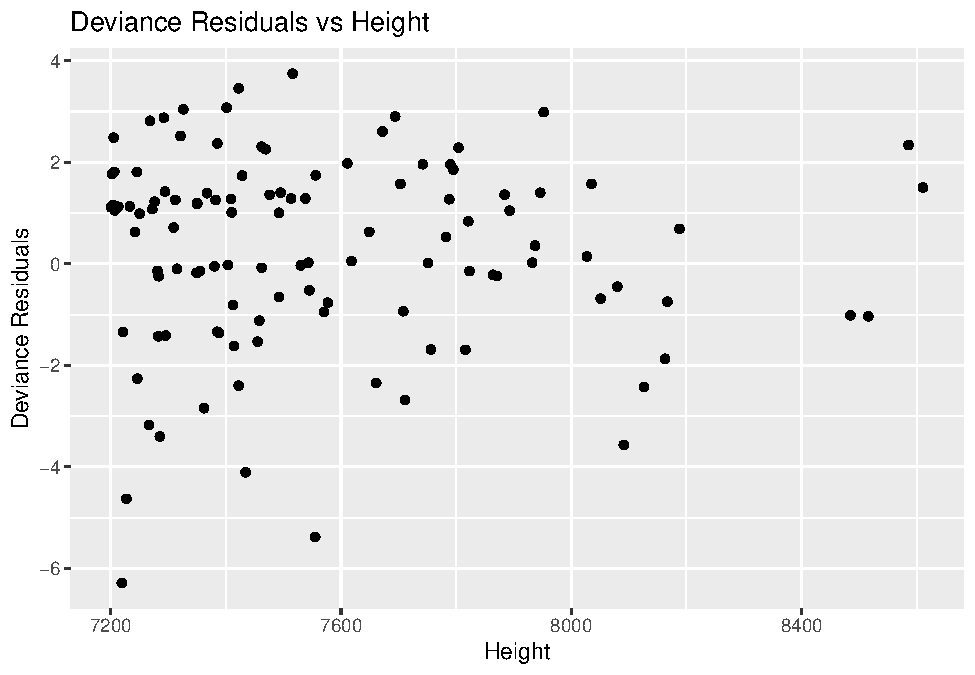
\includegraphics{TMA4315_comp_ex_2_files/figure-latex/unnamed-chunk-3-1.pdf}

\begin{Shaded}
\begin{Highlighting}[]
\CommentTok{\# Plotting deviance residuals against prominence}
\FunctionTok{ggplot}\NormalTok{(plot\_data, }\FunctionTok{aes}\NormalTok{(}\AttributeTok{x =}\NormalTok{ Prominence, }\AttributeTok{y =}\NormalTok{ DevRes)) }\SpecialCharTok{+} \FunctionTok{geom\_point}\NormalTok{() }\SpecialCharTok{+} \FunctionTok{labs}\NormalTok{(}\AttributeTok{x =} \StringTok{"Prominence"}\NormalTok{,}
    \AttributeTok{y =} \StringTok{"Deviance Residuals"}\NormalTok{, }\AttributeTok{title =} \StringTok{"Deviance Residuals vs Prominence"}\NormalTok{)}
\end{Highlighting}
\end{Shaded}

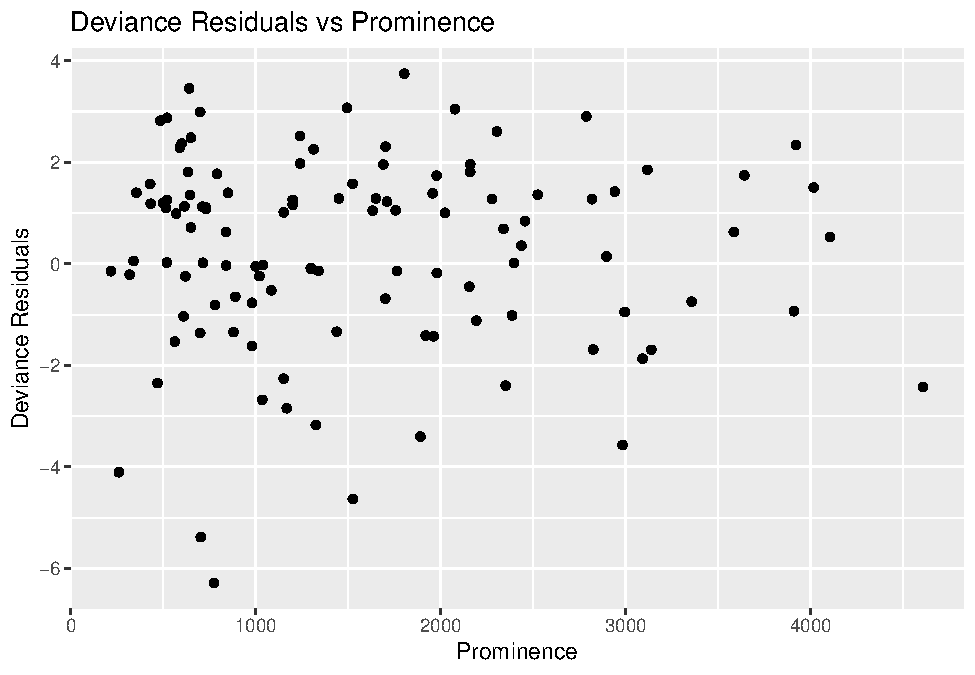
\includegraphics{TMA4315_comp_ex_2_files/figure-latex/unnamed-chunk-3-2.pdf}

\hypertarget{part-2}{%
\section{Part 2}\label{part-2}}

\begin{Shaded}
\begin{Highlighting}[]
\NormalTok{filepath }\OtherTok{\textless{}{-}} \StringTok{"https://www.math.ntnu.no/emner/TMA4315/2023h/eliteserien2023.csv"}
\NormalTok{eliteserie }\OtherTok{\textless{}{-}} \FunctionTok{read.csv}\NormalTok{(}\AttributeTok{file =}\NormalTok{ filepath)}

\NormalTok{NGames }\OtherTok{\textless{}{-}} \FunctionTok{table}\NormalTok{(}\FunctionTok{c}\NormalTok{(eliteserie}\SpecialCharTok{$}\NormalTok{home[}\SpecialCharTok{!}\FunctionTok{is.na}\NormalTok{(eliteserie}\SpecialCharTok{$}\NormalTok{yh)], eliteserie}\SpecialCharTok{$}\NormalTok{away[}\SpecialCharTok{!}\FunctionTok{is.na}\NormalTok{(eliteserie}\SpecialCharTok{$}\NormalTok{yh)]))}
\NormalTok{RangeofGames }\OtherTok{\textless{}{-}} \FunctionTok{range}\NormalTok{(NGames)}
\end{Highlighting}
\end{Shaded}

\hypertarget{a-1}{%
\subsection{a)}\label{a-1}}

In this case we have two team categories which can score M goals, where \(M = \max_{ij}{O_{ij}}\), \(\mathbf{O} \in \mathbb{R}^{2\times M}\) is the matrix representing the contingency table. The matrix of expected frequencies, whose entries are given by
\begin{equation*}
  E_{ij} = \frac{\sum_p{\mathbf{O}_{ip}} + \sum_k{\mathbf{O}_{kj}}}{\sum_{p, k}{\mathbf{O}_{pk}}}
\end{equation*}
can be written in matrix form as
\begin{equation}
  \mathbf{E} = \frac{\mathbf{O}\bm{1}_M\bm{1}_2^T\mathbf{O}}{\bm{1}^T_M\mathbf{O}\bm{1}_2}
  \label{eq:expfreq}
\end{equation}
where \(\bm{1}_k \in \mathbb{R}^k\) is the k-dimensional vector of ones. Using the definition of \(\mathbf{O}\) and Equation @ref\{eq:expfreq\}, the \(\chi^2\)-test can be written
\begin{equation}
  \chi^2 = \sum_{i, j}{\frac{\mathbf{O}_{ij} - \mathbf{E}_{ij}}{\mathbf{E}_{ij}}} \sim \chi^2_{1, M-1}
\end{equation}

\begin{Shaded}
\begin{Highlighting}[]
\CommentTok{\# O \textless{}{-} rbind(table(eliteserie$yh), table(eliteserie$ya)) O[2,}
\CommentTok{\# (max(eliteserie$ya)+1):max(eliteserie$yh)] \textless{}{-} 0}
\CommentTok{\# max(eliteserie$ya)}
\end{Highlighting}
\end{Shaded}


\end{document}
